\documentclass[tikz,border=8pt]{standalone}
% Shared look for every TikZ diagram. Load with \input{../../tools/tikz-style.tex}
\usepackage[T1]{fontenc}
\usepackage{lmodern}
\renewcommand{\sfdefault}{lmr}  % diagrams use the same serif as the text
\usetikzlibrary{arrows.meta, positioning, shapes.geometric, calc, fit, backgrounds}
\definecolor{cblue}{HTML}{4C78A8}
\definecolor{corange}{HTML}{F58518}
\definecolor{cgreen}{HTML}{54A24B}
\definecolor{cred}{HTML}{E45756}
\definecolor{cpurple}{HTML}{B279A2}
\definecolor{cgrey}{HTML}{6B6B6B}
\tikzset{
  every picture/.style={font=\sffamily, line width=1.2pt},
  box/.style={draw=#1, fill=#1!12, rounded corners=4pt, align=center, inner sep=7pt, minimum height=1.1cm},
  box/.default=cgrey,
  arrow/.style={-{Stealth[length=3mm]}, draw=cgrey, line width=1.4pt},
  title/.style={font=\sffamily\bfseries\Large},
  note/.style={font=\sffamily\small, text=cgrey, align=center},
}
\AtBeginDocument{\hyphenpenalty=10000 \exhyphenpenalty=10000}

\begin{document}
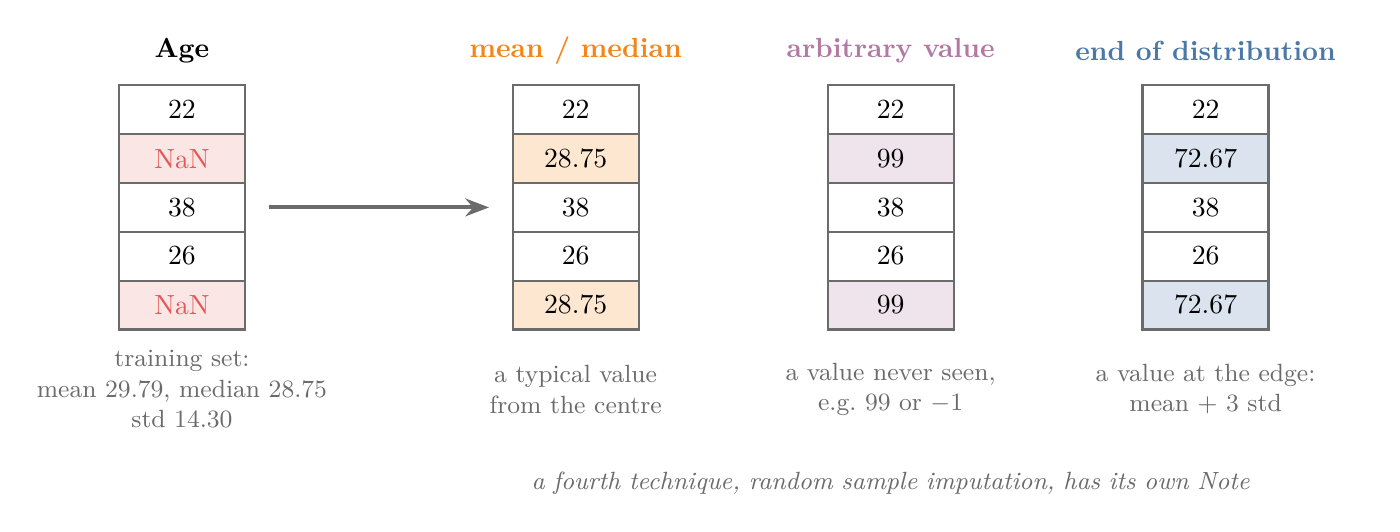
\begin{tikzpicture}[cell/.style={draw=cgrey, line width=0.8pt, minimum width=1.6cm, minimum height=0.62cm, font=\sffamily}]
  % a column with gaps
  \node[font=\sffamily\bfseries] at (0,0.75) {Age};
  \foreach \v/\i in {22/0, 38/2, 26/3} \node[cell] at (0,-0.62*\i) {\v};
  \foreach \i in {1,4} \node[cell, fill=cred!15, text=cred] at (0,-0.62*\i) {NaN};
  \node[note] at (0,-3.55) {training set:\\ mean 29.79, median 28.75\\ std 14.30};
  % three ways to fill it
  \foreach \x/\a/\b/\col/\t/\s in {
      5/28.75/28.75/corange/{mean / median}/{a typical value\\ from the centre},
      9/99/99/cpurple/{arbitrary value}/{a value never seen,\\ e.g.\ 99 or $-1$},
      13/72.67/72.67/cblue/{end of distribution}/{a value at the edge:\\ mean + 3 std}} {
    \node[font=\sffamily\bfseries, text=\col] at (\x,0.75) {\t};
    \node[cell] at (\x,0) {22};
    \node[cell, fill=\col!20] at (\x,-0.62) {\a};
    \node[cell] at (\x,-1.24) {38};
    \node[cell] at (\x,-1.86) {26};
    \node[cell, fill=\col!20] at (\x,-2.48) {\b};
    \node[note, text width=3.6cm] at (\x,-3.55) {\s};
  }
  \draw[arrow] (1.1,-1.24) -- (3.9,-1.24);
  \node[note, font=\sffamily\small\itshape, text width=12cm] at (9,-4.75) {a fourth technique, random sample imputation, has its own Note};
\end{tikzpicture}
\end{document}
